\chapter{Inclusion--Exclusion Principle}
\index{Inclusion--Exclusion Principle}

\section{Why We Need It}
When we count things in two groups, it is easy to accidentally count some
objects twice.

For example, suppose:
\begin{itemize}
  \item set \(A\) is students who play football;
  \item set \(B\) is students who play basketball.
\end{itemize}

If we do \(|A| + |B|\), students who play \emph{both} sports are counted twice.
So we must subtract the overlap once.

\section{Two-Set Formula}
For two finite sets \(A\) and \(B\), the inclusion--exclusion principle says
\[
  |A \cup B| = |A| + |B| - |A \cap B|.
\]

In words:
\begin{enumerate}
  \item include \(|A|\),
  \item include \(|B|\),
  \item exclude the overlap \(|A \cap B|\) once.
\end{enumerate}

\section{A Venn Diagram}
Figure~\ref{fig:venn-two-sets} shows the two-set case.  The overlapping region
\(A \cap B\) is exactly the part that would be double-counted if we used
\(|A|+|B|\) only.

\begin{figure}[htbp]
  \centering
  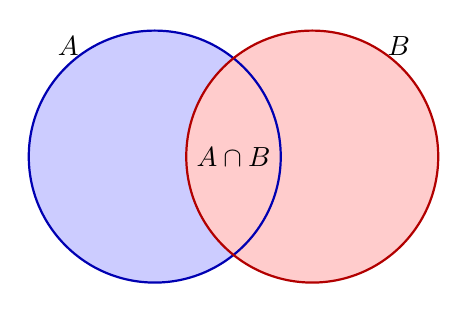
\begin{tikzpicture}[scale=1.0]
    \fill[blue!20] (-1.0,0) circle (1.6);
    \fill[red!20]  (1.0,0)  circle (1.6);
    \draw[thick, blue!70!black] (-1.0,0) circle (1.6);
    \draw[thick, red!70!black]  (1.0,0)  circle (1.6);
    \node at (-2.1,1.4) {\(A\)};
    \node at (2.1,1.4) {\(B\)};
    \node at (0,0) {\(A\cap B\)};
  \end{tikzpicture}
  \caption{Venn diagram for two sets \(A\) and \(B\).}
  \label{fig:venn-two-sets}
\end{figure}

\section{Three Sets}
For three sets \(A,B,C\), the same idea continues:
\[
  |A\cup B\cup C|
  = |A|+|B|+|C|
  - |A\cap B|-|A\cap C|-|B\cap C|
  + |A\cap B\cap C|.
\]

Why the last \(+\) term?
\begin{itemize}
  \item First we add \(|A|+|B|+|C|\): overlaps are overcounted.
  \item Then we subtract pairwise overlaps: this fixes most double counting.
  \item But the center region \(A\cap B\cap C\) was subtracted too many times,
        so we add it back once.
\end{itemize}

\section{From Three Sets to the General Pattern}
The jump from three sets to \(n\) sets is just the same correction process,
repeated one level further each time.

Think about an element \(x\) that belongs to exactly \(r\) of the sets
\(A_1,\dots,A_n\).  In the formula, this element is counted:
\begin{itemize}
  \item \(+\binom{r}{1}\) times in the ``single-set'' part,
  \item \(-\binom{r}{2}\) times in the pair-intersection part,
  \item \(+\binom{r}{3}\) times in the triple-intersection part,
  \item and so on, with alternating signs.
\end{itemize}

So the net coefficient of \(x\) becomes
\[
  \binom{r}{1} - \binom{r}{2} + \binom{r}{3} - \cdots + (-1)^{r+1}\binom{r}{r}.
\]
By the binomial identity \((1-1)^r=0\), this alternating sum equals \(1\).
That means every element in the union is counted exactly once, no matter how
many sets contain it.

This is the key reason the general formula works: each stage corrects the
over-correction made by the previous stage, and the alternating signs are
forced by this logic.

\section{General Formula}
For \(n\) sets \(A_1,\dots,A_n\):
\[
  \left|\bigcup_{i=1}^{n} A_i\right|
  =
  \sum_{i=1}^{n}|A_i|
  - \sum_{1\le i<j\le n}|A_i\cap A_j|
  + \sum_{1\le i<j<k\le n}|A_i\cap A_j\cap A_k|
  - \cdots
  + (-1)^{n+1}\left|\bigcap_{i=1}^{n}A_i\right|.
\]

The last sign is \(+\) when \(n\) is odd and \(-\) when \(n\) is even, exactly
following the alternating pattern.

Pattern to remember:
\begin{itemize}
  \item add single sets,
  \item subtract pair intersections,
  \item add triple intersections,
  \item subtract quadruple intersections,
  \item continue alternating signs.
\end{itemize}

\section{Why It Matters}
Inclusion--exclusion is a core counting tool in combinatorics and probability.
It appears in many topics, such as:
\begin{itemize}
  \item counting surjective functions,
  \item coupon collector formulas,
  \item probability of ``at least one event happens.''
\end{itemize}

Once you understand the two-set picture, the general formula is the same idea:
correct over-counting by alternating subtraction and addition.

